
% Inbuilt themes in beamer
\documentclass{beamer}

% Theme choice:
% \usetheme{CambridgeUS}
\usetheme{Darmstadt}
\usepackage{svg}

% Title page details: 
\title{Extracción automática de argumentos en textos de opinión en la prensa cubana} 
\author{Luis Ernesto Ibarra Vázquez}
\institute{Universidad de La Habana}
\date{13 de diciembre del 2022}
\logo{
\includegraphics[keepaspectratio=true,height=2cm,width=2cm]{Graphics/uhlogo.pdf}}


\begin{document}

% Title page frame
\begin{frame}
    \titlepage 
\end{frame}

% Remove logo from the next slides
\logo{}

% % Outline frame
% \begin{frame}{Outline}
%     \tableofcontents
% \end{frame}

\section{Introducción}
\begin{frame}{Argumentación}
    \begin{block}{Argumentación}
        La argumentación es una actividad verbal, social y racional destinada a convencer
        a un crítico razonable de la aceptabilidad de un punto de vista mediante la presentación 
        de una constelación de proposiciones que justifican o refutan la proposición
        expresada en el punto de vista.
    \end{block}
    \pause 
    \begin{block}{Extracción de Argumentos}
        La Extracción de Argumentos nace como la rama del Procesamiento de Lenguaje Natural encargada del
        estudio de métodos para la extracción automática de las \textbf{estructuras argumentativas}
        de los textos y su posterior procesamiento.
    \end{block}
\end{frame}
\begin{frame}{Extracción de argumentos: Partes y tareas}
    % Las estructuras argumentativas están compuestas por ...
    % Empezar a decir las definiciones de UDA.
    \begin{block}{Estructuras Argumentativas}
        \begin{itemize}
            \pause
            \item Unidades de discuso argumentativas (UDA).
            \pause
            \item Relaciones entre las UDAs.
        \end{itemize}
    \end{block}
    \pause
    % Las tareas de la EA son ...
    \begin{block}{Tareas de extracción de argumentos}
        \begin{itemize}
            \pause
            \item Extracción de las UDAs.
            \pause
            \item Clasificación de las UDAs.
            \pause
            \item Extracción de las relaciones entre las UDAs.
            \pause
            \item Clasificación de las relaciones entre las UDAs.
        \end{itemize}
    \end{block}
\end{frame}
\begin{frame}{Estructuras argumentativas como grafo}
    \includesvg[scale=.6]{Graphics/Estructuras_argumentativas.svg}
\end{frame}

\section{Propuesta}

\begin{frame}{Objetivos y propuesta}
    % \textbf{Objetivo:}
    \begin{block}{Objetivo}
        \pause
        Proponer un algoritmo para la extracción y
        análisis de estructuras argumentativas en textos de la prensa cubana.
    \end{block}
    \pause
    \begin{block}{Propuesta}
        \pause
        \begin{itemize}
            \item Dos modelos de aprendizaje profundo para:
            \begin{enumerate}
                \pause
                \item Extracción y clasificación de UDAs.
                \pause
                \item Extracción y clasificación de relaciones.
            \end{enumerate}
            % NOTA: Decir los problemas de falta de datos al español
            \pause
            \item Proyección de conjuntos de datos al español para el entrenamiento de los modelos
            propuestos. 
        \end{itemize}
    \end{block}
\end{frame}

\begin{frame}{Segmentación y clasificación de UDAs}
    \begin{columns}
        \begin{column}{0.10\textwidth}
            \begin{block}{}
                Texto
            \end{block}
        \end{column}
        \begin{column}<2->{0.01\textwidth}
            \begin{math}
                \Rightarrow
            \end{math}
        \end{column}
        \begin{column}<3->{0.30\textwidth}
            \begin{block}{}
                Segmentación y clasificación de UDAs.
            \end{block}
        \end{column}
        \begin{column}<4->{0.01\textwidth}
            \begin{math}
                \Rightarrow
            \end{math}
        \end{column}
        \begin{column}<5->{0.25\textwidth}
            \includesvg[scale=0.3]{Graphics/UDAs.svg}
        \end{column}
    \end{columns}

    \vspace{1cm}

    \begin{columns}[T]
        \begin{column}<2->{0.5\textwidth}
            Procesamiento de entrada:
            \begin{itemize}
                \item Tokenización.
                \item Anotación de las partes de la oración.
                \item Embeddings.
            \end{itemize}
        \end{column}
        \begin{column}<4->{0.5\textwidth}
            Procesamiento de salida:
            \begin{itemize}
                \item Arreglar el formato BIOES de las secuencias.
                \item Asignar una sola clasificación a cada segmento.
            \end{itemize}
        \end{column}
    \end{columns}
\end{frame}

\begin{frame}{Modelo de segmentación y clasificación de UDAs TODO}
    % \begin{columns}
    %     \begin{column}{0.5\textwidth}<1->
    %         \begin{center}
    %             \includesvg[scale=0.4]{Graphics/Modelo_segmenter_uda1.svg}
    %         \end{center}
    %     \end{column}
    %     \begin{column}{0.5\textwidth}<2->
    %         \begin{center}
    %             \includesvg[scale=0.4]{Graphics/Modelo_segmenter_uda2.svg}
    %         \end{center}
    %     \end{column}
    % \end{columns}
    \begin{onlyenv}<1>
        \begin{center}
            \includesvg[scale=0.4]{Graphics/Modelo_segmenter_uda1.svg}
        \end{center}
    \end{onlyenv}
    
    \begin{onlyenv}<2>
        \begin{center}
            \includesvg[scale=0.4]{Graphics/Modelo_segmenter_uda2.svg}
        \end{center}
    \end{onlyenv}
    % \begin{columns}
    %     \begin{column}{0.25\textwidth}
    %         Texto de ejemplo \\
    %         \begin{center}
    %             \begin{math}
    %                 \Downarrow
    %             \end{math}
    %         \end{center}
    %         \begin{block}{}
    %             Embeddings (GloVe, Char-Embeddings, POS)
    %         \end{block}
    %         \begin{center}
    %             \begin{math}
    %                 \Downarrow
    %             \end{math}
    %         \end{center}
    %         \begin{block}{}
    %             Procesamiento (BiLSTM, Capas densas)
    %         \end{block}
    %         \begin{center}
    %             \begin{math}
    %                 \Downarrow
    %             \end{math}
    %         \end{center}
    %         \begin{block}{}
    %             Clasificación (CRF)
    %         \end{block}
    %         \begin{center}
    %             \begin{math}
    %                 \Downarrow
    %             \end{math}
    %         \end{center}
    %         \begin{block}{}
    %             Texto anotado BIO
    %         \end{block}
    %     \end{column}
    %     % Usar \only<NUMERO>{Texto} para las explicaciones
    %     \begin{column}{0.25\textwidth}
    %         \begin{block}{}
    %             Bloque1
    %         \end{block}
    %         \begin{center}
    %             \begin{math}
    %                 \Downarrow
    %             \end{math}
    %         \end{center}
    %         \begin{block}{}
    %             Bloque2
    %         \end{block}
    %     \end{column}
    % \end{columns}
\end{frame}

\begin{frame}{Extracción y clasificación de relaciones}

    \begin{columns}
        \begin{column}{0.25\textwidth}
            \includesvg[scale=0.2]{Graphics/UDAs.svg}
        \end{column}
        \begin{column}<2->{0.01\textwidth}
            \begin{math}
                \Rightarrow
            \end{math}
        \end{column}
        \begin{column}<3->{0.30\textwidth}
            \begin{block}{}
                Extracción y clasificación de las relaciones.
            \end{block}
        \end{column}
        \begin{column}<4->{0.01\textwidth}
            \begin{math}
                \Rightarrow
            \end{math}
        \end{column}
        \begin{column}<5->{0.25\textwidth}
            \includesvg[scale=0.2]{Graphics/UDAs_relacionadas.svg}
        \end{column}
    \end{columns}

    \vspace{1cm}

    \begin{columns}[T]
        \begin{column}<2->{0.5\textwidth}
            Procesamiento de entrada:
            \begin{itemize}
                \item Tokenización.
                \item Embeddings.
                \item Creación de tuplas conteniendo la UDA fuente y la UDA objetivo y distancia argumentativa.
            \end{itemize}
        \end{column}
        \begin{column}<4->{0.5\textwidth}
            Procesamiento de salida:
            \begin{itemize}
                \item Asignar etiqueta a la relación en dependencia del resultado.
            \end{itemize}
        \end{column}
    \end{columns}
\end{frame}

\begin{frame}{Modelo de extracción y clasificación de relaciones}
    \begin{onlyenv}<1-2>
        \begin{columns}
            \begin{column}<1->{0.5\textwidth}
                \begin{center}
                    \includesvg[scale=0.4]{Graphics/Modelo_link_prediction_1.svg}
                \end{center}
            \end{column}
            \begin{column}<2->{0.5\textwidth}
                \begin{center}
                    \includesvg[scale=0.4]{Graphics/Modelo_link_prediction_2.svg}
                \end{center}
            \end{column}
        \end{columns}
    \end{onlyenv}
    \begin{onlyenv}<3>
        \begin{center}
            \includesvg[scale=0.40]{Graphics/Modelo_link_prediction_3.svg}
        \end{center}
    \end{onlyenv}
\end{frame}

\section{Experimentación}

% NOTA: Dada la falta de un corpus en el dominio de las cartas a la direccion se
% entrenó el modelo propuesto con diferentes conjuntos de datos.
% El modelo aprende el criterio de segmentación y clasificación de las UDAs y de las
% relaciones directamente del conjunto de datos.
% Destacar el desbalance de los datos.
\begin{frame}{Conjuntos de datos}
    \textbf{Conjuntos de datos:}
    \begin{itemize}
        \item<2-> Ensayos Argumentativos.
        \item<3-> Cornell eRulemaking Corpus (CDCP).
        \item<4-> Abstracts Randomized Control Trials (AbsTRCT).
    \end{itemize}
    \vspace{1cm}
    \uncover<2->{\textbf{Caractecrísticas:}}
    \begin{itemize}
        \item<2-> Documentos: \only<2>{286 textos}\only<3>{731 comentarios}\only<4>{500 documentos}
        \item<2-> Segmentado por: \only<2>{Cláusula}\only<3>{Oración}\only<4>{Oración}
        \item<2-> Clasificación de UDAs: \only<2>{Major claim (12 \%), claim (25 \%) y premise (63 \%)}\only<3>{Policy (17 \%), value (45 \%), fact (16\%), testimony (21 \%)y reference (1 \%)}\only<4>{Major claim (3 \%), claim (30 \%) y premise (67 \%)}
        \item<2-> Clasificación de relaciones: \only<2>{Attack (6 \%) y support (94 \%)}\only<3>{Reason (97 \%) y evidence (3 \%)}\only<4>{Support (85 \%), partial-attack (12 \%) y attack (3 \%)}
    \end{itemize}
\end{frame}

\begin{frame}{Selección del modelo de segmentación}
    \begin{table}
        \begin{center}
            \begin{tabular}{|l|c|c|c|c|c|c|} \hline
            Modelos 		& POS       & Char-CNN  & Char-LSTM & Res       & Norm      & Densa  \\ \hline
            Modelo 1		& $\times$	& $\times$    & $\times$    & $\times$	& $\times$    & $\times$ \\ \hline
            Modelo 2		& $\times$	& $\checkmark$    & $\checkmark$    & $\checkmark$	& $\checkmark$    & $\times$ \\ \hline
            Modelo 3		& $\checkmark$	& $\checkmark$    & $\checkmark$    & $\checkmark$	& $\checkmark$    & $\times$ \\ \hline
            \textbf<2->{Modelo 4}		& $\checkmark$	& $\checkmark$    & $\checkmark$    & $\checkmark$	& $\checkmark$    & $\checkmark$ \\ \hline
            \end{tabular}
        \caption{Variantes de arquitectura de los modelos de segmentación de UDA.}\label{table:segmenter_architecture_table}
        \end{center}
    \end{table}
    \begin{onlyenv}<3->
        \begin{table}
            \begin{center}
                \scalebox{0.85}{
                \begin{tabular}{|l|c|c|c|c|} \hline
                Corpus		            & Macro F1	        & \emph{Accuracy}     & 100\%F1       & 50\%F1  	     \\ \hline
                Ensayos Argumentativos  & 0,56 / 0,82		& 0,77 / 0,89	      & 0,72 / 0,81   & 0,83 / 0,94      \\ \hline
                CDCP		            & 0,45 / 0,56		& 0,66 / 0,96	      & 0,61 / 0,82   & 0,68 / 0,93      \\ \hline
                AbsTRCT	                & 0,50 / 0,79		& 0,87 / 0,91	      & 0,61 / 0,66   & 0,75 / 0,82      \\ \hline
                \end{tabular}
                }
            \caption{Métricas del segmentador en su versión completa y BIOES.}\label{table:test_metrics_segmenter}
            \end{center}
        \end{table}
    \end{onlyenv}
\end{frame}

\begin{frame}{Selección del modelo de predicción de enlace}
    \begin{table}
        \begin{center}
            \scalebox{0.7}{
            \begin{tabular}{|l|c|c|c|c|c|c|} \hline
            Modelos   	             & Atención      & Pooling  & \emph{Dropout}   & T. de aprendizaje & Paciencia & Devolver mejores     \\ \hline
            Modelo 1            	 & $\times$	     &  5       & 0,5              & 0,0015            & 10	       & $\checkmark$        \\ \hline
            \textbf<2->{Modelo 2}    & $\times$	 	 & 10       & 0,1              & 0,003             & 5	       & $\times$            \\ \hline
            Modelo 3	             & $\checkmark$	 &  1       & 0,1              & 0,003             & 5	       & $\times$            \\ \hline
            Modelo 4	             & $\checkmark$	 &  1       & 0,5              & 0,0015            & 10	       & $\checkmark$        \\ \hline
            \end{tabular}
            }
        \caption{Variantes de arquitectura de los modelos de predicción de enlaces.}\label{table:link_predictor_architecture_table}
        \end{center}
    \end{table}
    \begin{onlyenv}<3->
        \begin{table}
            \begin{center}
                \scalebox{0.7}{
                \begin{tabular}{|l|c|c|c|c|} \hline
                Corpus		            & Macro F1 Clasif. & \emph{Acc.} Clasif. & Macro F1 Enlace & \emph{Acc.} Enlace \\ \hline
                Ensayos Argumentativos  & 0,33	   & 0,57            & 0,68	    		& 0,75	  \\ \hline
                CDCP		            & 0,37	   & 0,63	         & 0,79	    		& 0,68	  \\ \hline
                AbsTRCT	                & 0,39	   & 0,61	         & 0,83	    		& 0,74	  \\ \hline
                \end{tabular}
                }
            \caption{Métricas de predicción de relaciones de las pruebas del predictor de enlace.}\label{table:test_relation_metrics_link_predictor}
            \end{center}
        \end{table}
    \end{onlyenv}
\end{frame}

\section{Conclusiones}

\begin{frame}{Resultados}
    Se anotaron las Cartas a la Dirección con los modelos entrenados en los diferentes conjuntos de datos 
    para determinar el modelo que se ajusta a los datos, llegando a las siguientes consideraciones luego de
    analizar un subconjunto 15 pares de cartas seleccionadas:
    
    \begin{itemize}
        \begin{onlyenv}<2-5>
            \item AbsTRCT:
            \begin{itemize}
                \item<3-> Todas las UDAs son clasificadas como Premisa.
                \item<4-> Existen pocas relaciones extraídas.
                \item<5-> La precisión de las relaciones de \textit{partial-attack} es baja.
            \end{itemize}
        \end{onlyenv}
        \begin{onlyenv}<6-10>
            \item Ensayos Persuasivos:
            \begin{itemize}
                \item<7-> Mejora en cuanto a la variedad de las clasificaciones de las UDAs.
                \item<8-> Posee problemas de segmentación en la que la UDA se queda incompleta.
                \item<9-> Posee una gran cantidad de falsos positivos en las relaciones.
                \item<10-> No se encuentran relaciones de \textit{attack} anotadas.
            \end{itemize}
        \end{onlyenv}
        \begin{onlyenv}<11->
            \item CDCP:
            \begin{itemize}
                \item<12-> Mejora en la segmentación 
                (Las oraciones tienden a formar mejores UDAs en este tipo de texto).
                \item<13-> Disminuye la cantidad de falsos positivos en las relaciones.
                \item<14-> No posee una relación de ataque entre sus candidatos.
            \end{itemize}
        \end{onlyenv}
    \end{itemize}
    \only<15>{Se selecciona este conjunto de datos para la anotación final de las Cartas a la Dirección}
\end{frame}

% NOTA: Decir las conclusiones mostrando capturas del software final. Streamlit, Brat
% - Se crearon modelos que permiten la extraccion automatica de las estructras argumentativas del texto
% capaz de acomodarse a diferentes definiciones de estas
% - Se anotaron las estructuras argumentativas de las Cartas a la Dirección con dichos modelos
% - Se visualizan dichos datos de tal forma que puedan ser modificados
\begin{frame}{Resultados}
    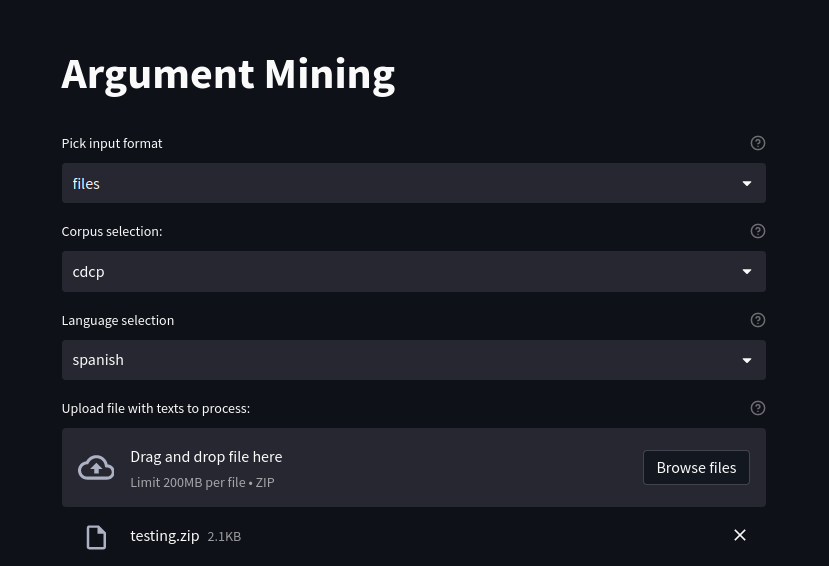
\includegraphics[keepaspectratio=true,height=\textheight,width=\textwidth]{Graphics/streamlit_app.png}<1>
    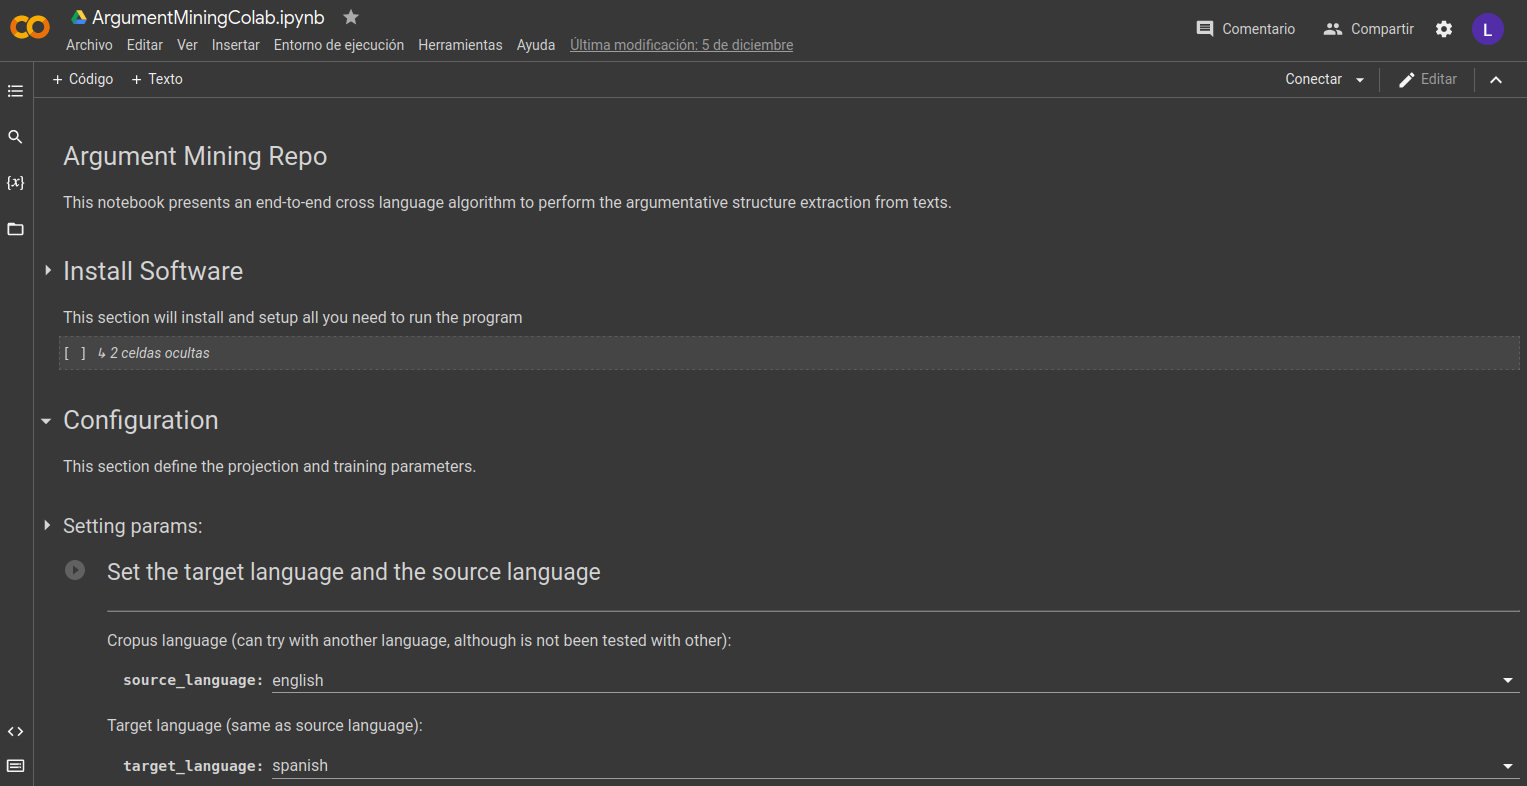
\includegraphics[keepaspectratio=true,height=\textheight,width=\textwidth]{Graphics/colab.png}<2>
    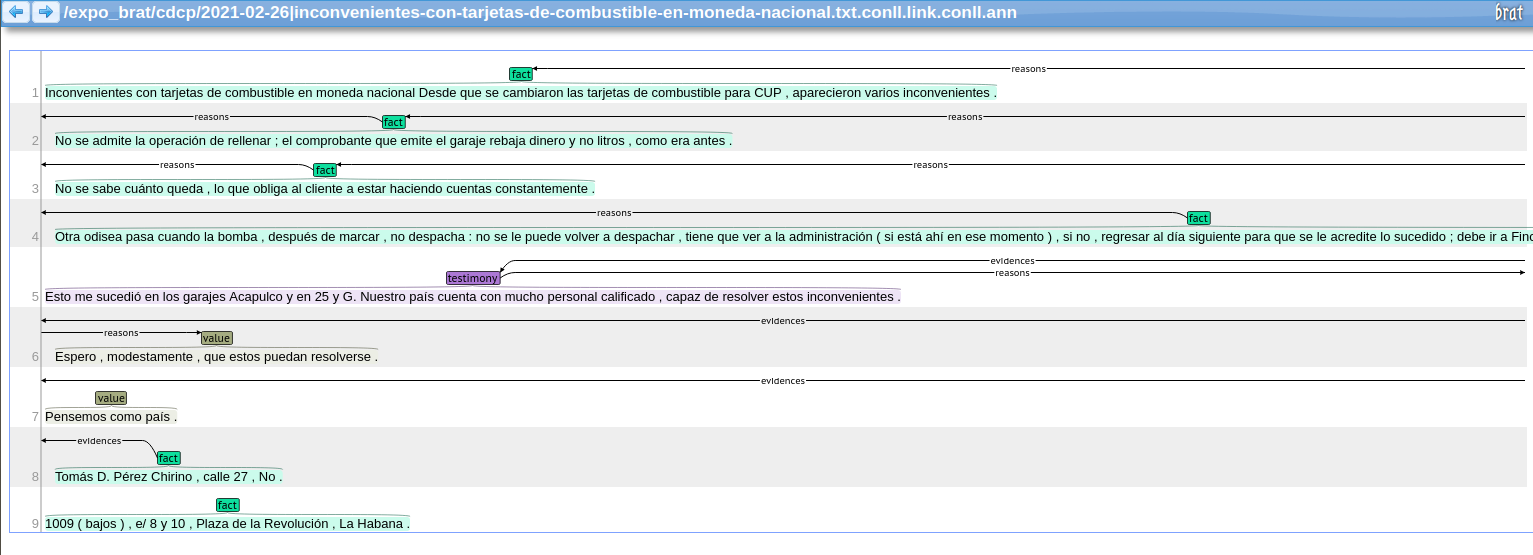
\includegraphics[keepaspectratio=true,height=\textheight,width=\textwidth]{Graphics/brat_cdcp_example.png}<3>
\end{frame}

\begin{frame}{Recomendaciones}
    \begin{itemize}
        \item<1-> Anotar las Cartas a la Dirección con las estructuras argumentativas por lingüístas.
        \item<2-> Aplicar el uso de otros \textit{embeddings}, como BERT, entrenados sobre el conjunto 
        de datos extraído.
        \item<3-> Proponer un modelo capaz de tomar en cuenta el contexto del texto completo para la
        predicción y clasificación de enlaces, por ejemplo \textit{Graph Neural Networks}.
    \end{itemize}    
\end{frame}

% Title page frame
\begin{frame}
    \titlepage 
\end{frame}

\begin{frame}{Preguntas del oponente?}
    
\end{frame}

\end{document}
